\documentclass[11pt]{report}

%-------------------------------------------------------------------------------------------------%

% PAQUETES

\usepackage[a4paper, right = 0.8in, left = 0.8in, top = 0.8in, bottom = 0.8in]{geometry}
\usepackage[utf8]{inputenc}
\usepackage[spanish]{babel}
\usepackage{amsmath,amsfonts,amssymb,amsthm}
\usepackage{multicol}
\usepackage{fouriernc}
\usepackage{enumitem}
\usepackage{mathtools} % Solo uso \underbracket
\usepackage{cellspace, tabularx, booktabs} % Líneas del título
\usepackage{parskip}
\usepackage{pdfpages}
\usepackage{cancel}

%-------------------------------------------------------------------------------------------------%

% AJUSTES GENERALES

\setlist[enumerate]{label={\textit{\alph*})}}

\makeatletter % Para quitar el espacio adicional que el paquete parskip añade al principio y al final de una demostración
\renewenvironment{proof}[1][\proofname]{\par
  \pushQED{\qed}%
  \normalfont \topsep\z@skip % <---- changed here
  \trivlist
  \item[\hskip\labelsep
        \itshape
    #1\@addpunct{.}]\ignorespaces
}{%
  \popQED\endtrivlist\@endpefalse
}
\makeatother

%-------------------------------------------------------------------------------------------------%

% COMANDOS PERSONALIZADOS

\newcommand{\N}{\mathbb N}
\newcommand{\Z}{\mathbb Z}
\newcommand{\Q}{\mathbb Q}
\newcommand{\R}{\mathbb R}
\newcommand{\C}{\mathbb C}

\newcommand{\pars}[1]{\left( #1 \right)} % Paréntesis de tamaño automático
\newcommand{\comment}[1]{}

%-------------------------------------------------------------------------------------------------%

% EJERCICIOS Y SOLUCIONES

\newtheorem{ejercicio}{Ejercicio}
\addto\captionsspanish{\renewcommand*{\proofname}{Solución}}

%-------------------------------------------------------------------------------------------------%

\begin{document}

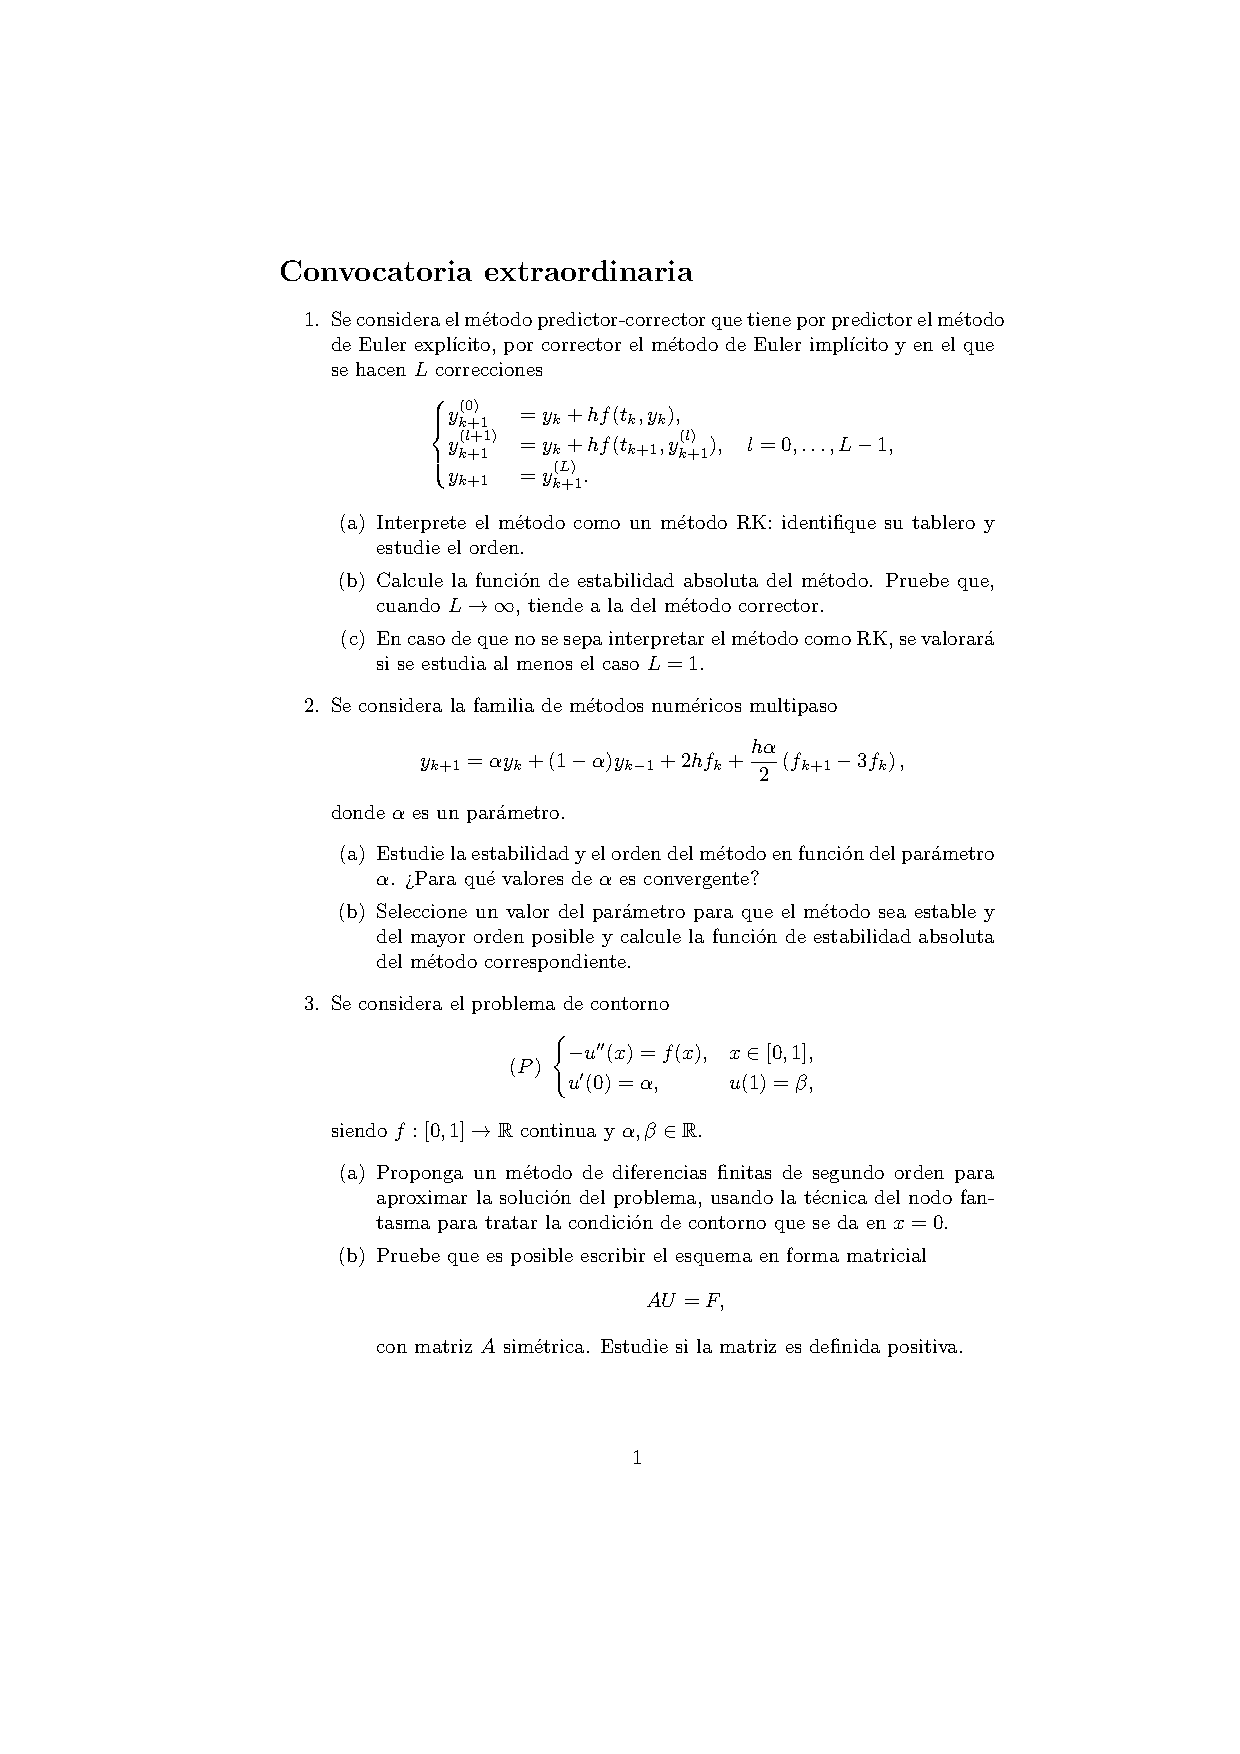
\includepdf[pages=-]{an_examen_2023-11.pdf}

%-------------------------------------------------------------------------------------------------%

% TÍTULO

\begin{center}

	\textbf{$-$ Resolución $-$}

\end{center}

%-------------------------------------------------------------------------------------------------%

\textbf{1. }

\begin{enumerate}
    \item El método dado puede escribirse como 
    \[\left\{ \begin{alignedat}{1}
        y_k^* &= y_k, \\
        y_{k}^{(0)} &= y_k+hf(t_k,y_k^*), \\
        y_{k}^{(l+1)} &= y_k+hf(t_k+h, y_{k}^{(l)}), \qquad l = 0,1,\mathellipsis,L-1, \\
        y_{k+1} &= y_{k}+hf(t_k+h,y_{k}^{(L-1)}),
    \end{alignedat} \right.\]
    que es un método de Runge-Kutta con tablero de Butcher

    \begin{center}
        \setlength\extrarowheight{2.5pt}
        \begin{tabular}{c|cccccc}
            0 & 0 & 0 & 0 & $\mathellipsis$ & 0 & 0 \\
            0 & 1 & 0 & 0 & $\mathellipsis$ & 0 & 0 \\
            1 & 0 & 1 & 0 & $\mathellipsis$ & 0 & 0 \\
            1 & 0 & 0 & 1 & $\mathellipsis$ & 0 & 0 \\
            $\vdots$ & $\vdots$ & $\vdots$ & $\vdots$ & $\ddots$ & $\vdots$ & $\vdots$ \\
            1 & 0 & 0 & 0 & $\mathellipsis$ & 1 & 0 \\ \hline
            & 0 & 0 & 0 & $\mathellipsis$ & 1 & 0 
        \end{tabular}
    \end{center}

    Sean $A,C \in \mathcal{M}_{L+2}(\R)$, $B \in \R^{n+2}$ las matrices del método. Es claro que que
    \[B^tE= 1,\]
    así que el método es de orden $1$. Además,
    \[B^tAE = \left(\begin{array}{ccccc}
        0 & 0 & \mathellipsis & 1 & 0 
    \end{array}\right)\left(\begin{array}{cccccc}
        0 & 0  & \mathellipsis & 0 & 0 & 0 \\
        1 & 0  & \mathellipsis & 0 & 0 & 0 \\
        0 & 1  & \mathellipsis & 0 & 0 & 0 \\
        \vdots & \vdots & \ddots & \vdots & \vdots & \vdots \\
        0 & 0 &  \mathellipsis & 1 & 0 & 0 \\
        0 & 0 &  \mathellipsis & 0 & 1 & 0
    \end{array}\right)\left(\begin{array}{c}
        1 \\
        1 \\
        1 \\
        \vdots \\
        1 \\
        1
    \end{array}\right) = \left(\begin{array}{cccccc}
        0 & \mathellipsis & 0 & 1 & 0 & 0 
    \end{array}\right)\left(\begin{array}{c}
        1 \\
        \vdots \\
        1 \\
        1 \\
        1 \\
        1
    \end{array}\right) = 1\]
    Como $B^tAE \neq \frac{1}{2}$, el método es de orden $1$.
    \item La función de estabilidad absoluta del método es
    \[R(\hat{h}) = \frac{|I-\hat{h}A+\hat{h}EB^t|}{|I-\hat{h}A|}\]
    Como $I-\hat{h}A$ es una matriz triangular inferior con diagonal llena de unos, su determinante es $1$. Además,
    \[\hat{h}EB^t = \left(\begin{array}{c}
        \hat{h} \\
        \vdots \\
        \hat{h} \\
        \hat{h} \\
        \hat{h}
    \end{array}\right)\left(\begin{array}{cccccc}
        0 & \mathellipsis & 0 & 1 & 0
    \end{array}\right) = \left(\begin{array}{ccccc}
        0 & \mathellipsis & 0 & \hat{h} & 0 \\
        0 & \mathellipsis & 0 & \hat{h} & 0 \\
        \vdots & \ddots & \vdots & \vdots & \vdots \\
        0 & \mathellipsis & 0 & \hat{h} & 0 \\
    \end{array}\right)\]
    Por tanto,
    \[I-\hat{h}A+\hat{h}EB^t = \left(\begin{array}{cccccc}
        1 & 0 & \mathellipsis & 0 & \hat{h} & 0 \\
        -\hat{h} & 1 &  \mathellipsis & 0 & \hat{h} & 0 \\
        0 & -\hat{h} &  \mathellipsis & 0 & \hat{h} & 0 \\
        \vdots & \vdots & \ddots & \vdots & \vdots & \vdots \\
        0 & 0 &  \mathellipsis & -\hat{h}& 1+\hat{h} & 0 \\
        0 & 0 &  \mathellipsis & 0 & 0 & 1
    \end{array}\right)\]
    Desarrollando el determinante por la última columna,
    \[|I-\hat{h}A+\hat{h}EB^t| = \left|\begin{array}{cccccc}
        1 & 0 & \mathellipsis & 0 & \hat{h} \\
        -\hat{h} & 1 &  \mathellipsis & 0 & \hat{h} \\
        0 & -\hat{h} &  \mathellipsis & 0 & \hat{h}  \\
        \vdots & \vdots & \ddots & \vdots & \vdots \\
        0 & 0 &  \mathellipsis & -\hat{h}& 1+\hat{h} \\
    \end{array}\right| \tag{$\ast$}\]
    Vamos a suponer por comodidad que $L$ es impar (para $L$ par será análogo), así que $L+1$ es par y al desarrollar por la última colummna obtenemos
    \[|I-\hat{h}A+\hat{h}EB^t| = \sum_{j=1}^{L}(-1)^j\hat{h}|A_j|+(1+\hat{h})|A_{L+1}|,\]
    donde, para $j=1,2,\mathellipsis,L+1$, la matriz $A_j$ resulta de eliminar en la matriz que aparece en $(\ast)$ la última columna y la fila $j$-ésima. Observamos que $A_j \in \mathcal{M}_L(\R)$ es una matriz triangular cuyos elementos diagonales son $1$ (aparece $j-1$ veces) y $-\hat{h}$ (aparece $L-j+1$ veces), deduciéndose que $|A_j| = (-\hat{h})^{L-j+1}$ y
    \[|I-\hat{h}A+\hat{h}EB^t| = \sum_{j=1}^{L}(-1)^{L+1}\hat{h}^{L-j+2}+1+\hat{h} = \sum_{j=1}^{L}\hat{h}^{L-j+2}+1+\hat{h}\]
    Reordenando los sumandos adecuadamente, concluimos que
    \[R(\hat{h}) = |I-\hat{h}A+\hat{h}EB^t| = \sum_{j=2}^{L+1}\hat{h}^j+1+\hat{h}=\sum_{j=0}^{L+1}\hat{h}^j\]
    Por tanto, siempre que $|\hat{h}|<1$,
    \[\lim_{L \to \infty} R(\hat{h}) = \sum_{j=0}^\infty \hat{h}^j = \frac{1}{1-\hat{h}},\]
    que es, milagrosamente, la función de estabilidad absoluta del método de Euler implícito.
\end{enumerate}

\textbf{2. }

\begin{enumerate}
    \item El primer polinomio característico del método es $\rho(z) = z^2-\alpha z+\alpha-1$. Se tiene que
    \[z^2-\alpha z+\alpha- 1 = 0 \iff z = \frac{\alpha\pm \sqrt{\alpha^2-4\alpha+4}}{2} = \frac{\alpha \pm \sqrt{(\alpha-2)^2}}{2} = \frac{\alpha \pm (\alpha-2)}{2} \iff z \in \{\alpha-1, 1\}\]
    El método es estable si y solo si las raíces de $\rho$ son de módulo menor que $1$ y las de módulo $1$ (si las hay) son simples. En este caso, el método es estable si y solo si $|\alpha-1|<1$ o $\alpha = 0$, o sea, si y solo si $\alpha \in [0,2)$.

    Estudiemos el orden. En primer lugar, los coeficientes del método son
    \[\alpha_0 = \alpha-1, \qquad \alpha_1=-\alpha, \qquad \alpha_2 = 1, \qquad \beta_0 = 0, \qquad \beta_1 = 2-\frac{3\alpha}{2}, \qquad \beta_2 = \frac{\alpha}{2}\]
    Se tiene que
    \[\sum_{j=0}^2 \alpha_j = 1-\alpha+\alpha-1 = 0\]
    Además,
    \[\sum_{j=0}^2 \alpha_j j =2-\alpha, \qquad \qquad  \sum_{j=0}^2 \beta_j = 2-\alpha\]
    Por tanto, el método es de orden $1$ independientemente del valor de $\alpha$. Como
    \[\sum_{j=0}^2 \alpha_j j^2 =4-\alpha, \qquad \qquad  2\sum_{j=0}^2 \beta_jj = 2\left(2-\frac{3\alpha}{2}+\alpha\right) = 4-\alpha,\]
    entonces el método es de orden $2$ independientemente de $\alpha$. Y como
    \[\sum_{j=0}^2 \alpha_j j^3 =8-\alpha, \qquad \qquad  3\sum_{j=0}^2 \beta_jj^2 = 3\left(2-\frac{3\alpha}{2}+2\alpha\right) =3 \left(2+\frac{\alpha}{2}\right) = 6+\frac{3\alpha}{2}\]
    Por tanto,
    \[\textup{ el método es de orden } 3 \iff 8-\alpha = 6+\frac{3\alpha}{2} \iff 16-2\alpha = 12+3\alpha \iff \alpha = \frac{4}{5}\]
    Veamos si el método es de orden $4$ para $\alpha = \frac{4}{5}$:
    \[\sum_{j=0}^2 \alpha_j j^4 =16-\alpha = \frac{76}{5}, \qquad \qquad 4\sum_{j=0}^2 \beta_jj^3 = 4\left(2-\frac{3\alpha}{2}+4\alpha\right) =4 \left(2+\frac{5\alpha}{2}\right) = 8+10\alpha = 16\]
    Por tanto, el método no es de orden $4$.

    El método es convergente si y solo si es estable y consistente, es decir, si y solo si $\alpha \in[0,2)$.

    \item Para que el método sea estable y del mayor orden posible hay que tomar $\alpha = \frac{4}{5}$. Hallemos el dominio de estabilidad absoluta del método. Se tiene que $\hat{h} \in D_A$ si y solo si todas las raíces de $\pi_{\hat{h}}$ tienen módulo menor que $1$, donde
    \[\pi_{\hat{h}}(z)=\rho(z)-\hat{h}\sigma(z), \qquad \qquad \rho(z)=z^2-\alpha z+\alpha-1, \qquad \qquad \sigma(z)=\frac{\alpha}{2}z^2+\left(2-\frac{3\alpha}{2}\right)z\]
    Se tiene que
    \[\pi_{\hat{h}}(z)=0 \iff \hat{h} = \frac{\rho(z)}{\sigma(z)} = \frac{z^2-\alpha z+\alpha-1}{\frac{\alpha}{2}z^2+\left(2-\frac{3\alpha}{2}\right)z}\]
\end{enumerate}

\end{document}